\documentclass[tikz]{standalone}

\usetikzlibrary{calc,positioning}

\tikzset{block/.style={%
  inner xsep=2mm,
  inner ysep=2mm,
  anchor=center,
  rounded corners,
  very thick,
  draw}}

\tikzset{link/.style={->,very thick,>=stealth,rounded corners}}


\begin{document}

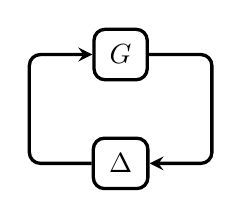
\begin{tikzpicture}
  \node (G)  [block] {$G$};
  \node (df) [block,below=7mm of G] {$\Delta$};
    
  \draw [link] (G) -- ($(G.east)+(8mm,0)$) -- ($(G.east |-  df)+(8mm,0)$) -- (df);
  \draw [link] (df) -- ($(G.west |- df)-(8mm,0)$) -- ($(G.west)-(8mm,0)$) -- (G);
\end{tikzpicture}

\end{document}